%------------------------------------------------
%	PACKAGES AND DOCUMENT CONFIGURATIONS
%------------------------------------------------
\documentclass[11pt]{article}
\usepackage{amsmath} % Required for some math elements
\usepackage{hyperref} 
\usepackage{xcolor}
\usepackage{lipsum} 
\usepackage{cite}
\usepackage{graphicx} % Required for the inclusion of images
\usepackage{algorithmic}
\usepackage{array}
\usepackage{bookmark}
\usepackage{listings}
\usepackage{amssymb}
\usepackage{enumitem}
\usepackage{pythonhighlight}
\usepackage[T1]{fontenc}
\usepackage{inconsolata}
\usepackage[margin=16mm]{geometry}
\usepackage[caption=false, font=footnotesize]{subfig}
\usepackage[active,tightpage]{preview}

\renewcommand{\PreviewBorder}{1in}
\newcommand{\Newpage}{\end{preview}\begin{preview}}

\newlist{steps}{enumerate}{1}
\setlist[steps, 1]{label = Step \arabic*:}

\hypersetup{ %color attributes of citation, link, etc.
    colorlinks=true,
    linkcolor=blue,
    filecolor=gray,      
    urlcolor=blue,
    citecolor=blue,
}

\newcommand{\matlab}{\textsc{Matlab }} %very important and totally necessary addition

\newcommand\Item[1][]{%
  \ifx\relax#1\relax  \item \else \item[#1] \fi
  \abovedisplayskip=0pt\abovedisplayshortskip=0pt~\vspace*{-\baselineskip}}

%----------------------------------
%	DOCUMENT INFORMATION
%----------------------------------
 
\title{ECEN321 : Hypothesis Testing \\ Lab 5 Submission}
\author{Daniel Eisen : 300447549}
\date{\today}

\begin{document}
\begin{preview}
\maketitle
%-----------------------------
%	DOCUMENT CONTENT
%-----------------------------
\section{Introduction}
 Regression is an approach to modelling the relationship between a dependent variable and one or more  independent variables. The case of one explanatory variable is called simple linear regression. This is what this lab attempts to demonstrate when analysing the relationship between time and average local temperature.

\section{Theory}
The correlation coefficient between the variables, denoted r, is first computed.
\begin{align*}
        r &= \frac{1}{n-1}\sum_{i = 1}^{n} \left(\frac{x_i-\bar{x}}{s_x} \right) \left(\frac{y_i-\bar{y}}{s_y}\right)\\\\
          &= \frac{\sum_{i = 1}^{n}  (x_i - \bar{x})(y_i - \bar{y})  }{\sqrt{\sum_{i = 1}^{n}  (x_i - \bar{x})^2(y_i - \bar{y})^2 }}\\
    \end{align*}
Then the estimators for the slope ($\beta_1$) and y-intercept ($\beta_0$) can be computed:


\begin{align*}
        \beta_1 &= \frac{\sum(y-\bar{y})(x-\bar{x})}{\sum(x-\bar{x})^2}\\
        \beta_0 &= \bar{y} - \beta_1 \bar{x}
\end{align*}

For Hypothesis testing, the p value can then be computed:
$$\frac{r\sqrt{n-2}}{1-r^2} \approx t^*(n-2)$$

\section{Results}
Regression was performed on data from Taipei,Taiwan see below in figure 1

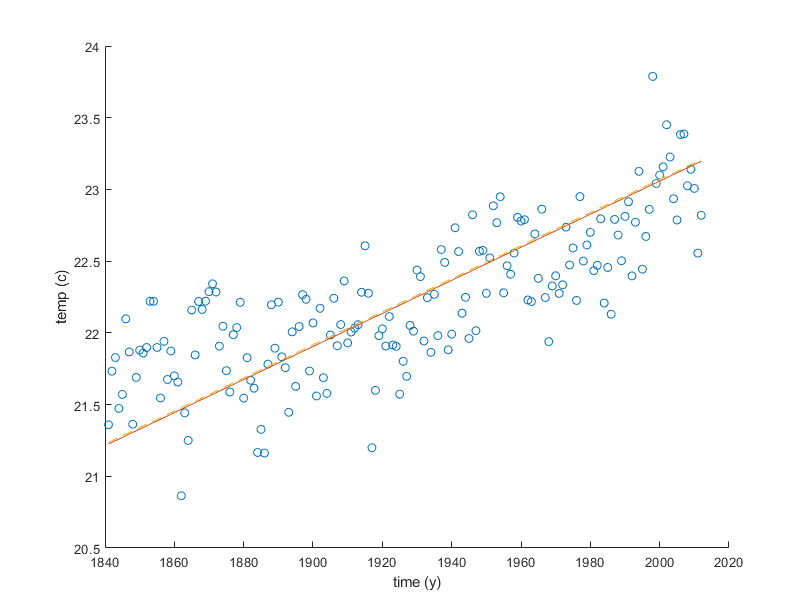
\includegraphics[width=\textwidth]{plt.png}
For null or r = 0:

Computeed $\beta_1$ = 0.0115 \\
95\% interval = 0.01149,0.011558 \\
R = 0.004715
t = 0.061472

\end{preview}
\end{document}